% defer/refcnt.tex

\section{Reference Counting}
\label{sec:defer:Reference Counting}

{ \scriptsize
\begin{verbbox}
 1 struct route_entry {
 2   atomic_t re_refcnt;
 3   struct route_entry *re_next;
 4   unsigned long addr;
 5   unsigned long iface;
 6   int re_freed;
 7 };
 8 struct route_entry route_list;
 9 DEFINE_SPINLOCK(routelock);
10
11 static void re_free(struct route_entry *rep)
12 {
13   ACCESS_ONCE(rep->re_freed) = 1;
14   free(rep);
15 }
16
17 unsigned long route_lookup(unsigned long addr)
18 {
19   int old;
20   int new;
21   struct route_entry *rep;
22   struct route_entry **repp;
23   unsigned long ret;
24
25 retry:
26   repp = &route_list.re_next;
27   rep = NULL;
28   do {
29     if (rep &&
30         atomic_dec_and_test(&rep->re_refcnt))
31       re_free(rep);
32     rep = ACCESS_ONCE(*repp);
33     if (rep == NULL)
34       return ULONG_MAX;
35     do {
36       if (ACCESS_ONCE(rep->re_freed))
37         abort();
38       old = atomic_read(&rep->re_refcnt);
39       if (old <= 0)
40         goto retry;
41       new = old + 1;
42     } while (atomic_cmpxchg(&rep->re_refcnt,
43                             old, new) != old);
44     repp = &rep->re_next;
45   } while (rep->addr != addr);
46   ret = rep->iface;
47   if (atomic_dec_and_test(&rep->re_refcnt))
48     re_free(rep);
49   return ret;
50 }
\end{verbbox}
}
\begin{figure}[bp]
\centering
\theverbbox
\caption{Reference-Counted Pre-BSD Routing Table Lookup}
\label{fig:defer:Reference-Counted Pre-BSD Routing Table Lookup}
\end{figure}

{ \scriptsize
\begin{verbbox}
 1 int route_add(unsigned long addr,
 2               unsigned long interface)
 3 {
 4   struct route_entry *rep;
 5
 6   rep = malloc(sizeof(*rep));
 7   if (!rep)
 8     return -ENOMEM;
 9   atomic_set(&rep->re_refcnt, 1);
10   rep->addr = addr;
11   rep->iface = interface;
12   spin_lock(&routelock);
13   rep->re_next = route_list.re_next;
14   rep->re_freed = 0;
15   route_list.re_next = rep;
16   spin_unlock(&routelock);
17   return 0;
18 }
19
20 int route_del(unsigned long addr)
21 {
22   struct route_entry *rep;
23   struct route_entry **repp;
24
25   spin_lock(&routelock);
26   repp = &route_list.re_next;
27   for (;;) {
28     rep = *repp;
29     if (rep == NULL)
30       break;
31     if (rep->addr == addr) {
32       *repp = rep->re_next;
33       spin_unlock(&routelock);
34       if (atomic_dec_and_test(&rep->re_refcnt))
35         re_free(rep);
36       return 0;
37     }
38     repp = &rep->re_next;
39   }
40   spin_unlock(&routelock);
41   return -ENOENT;
42 }
\end{verbbox}
}
\begin{figure}[bp]
\centering
\theverbbox
\caption{Reference-Counted Pre-BSD Routing Table Add/Delete}
\label{fig:defer:Reference-Counted Pre-BSD Routing Table Add/Delete}
\end{figure}

\begin{figure}[tb]
\centering
\resizebox{2.5in}{!}{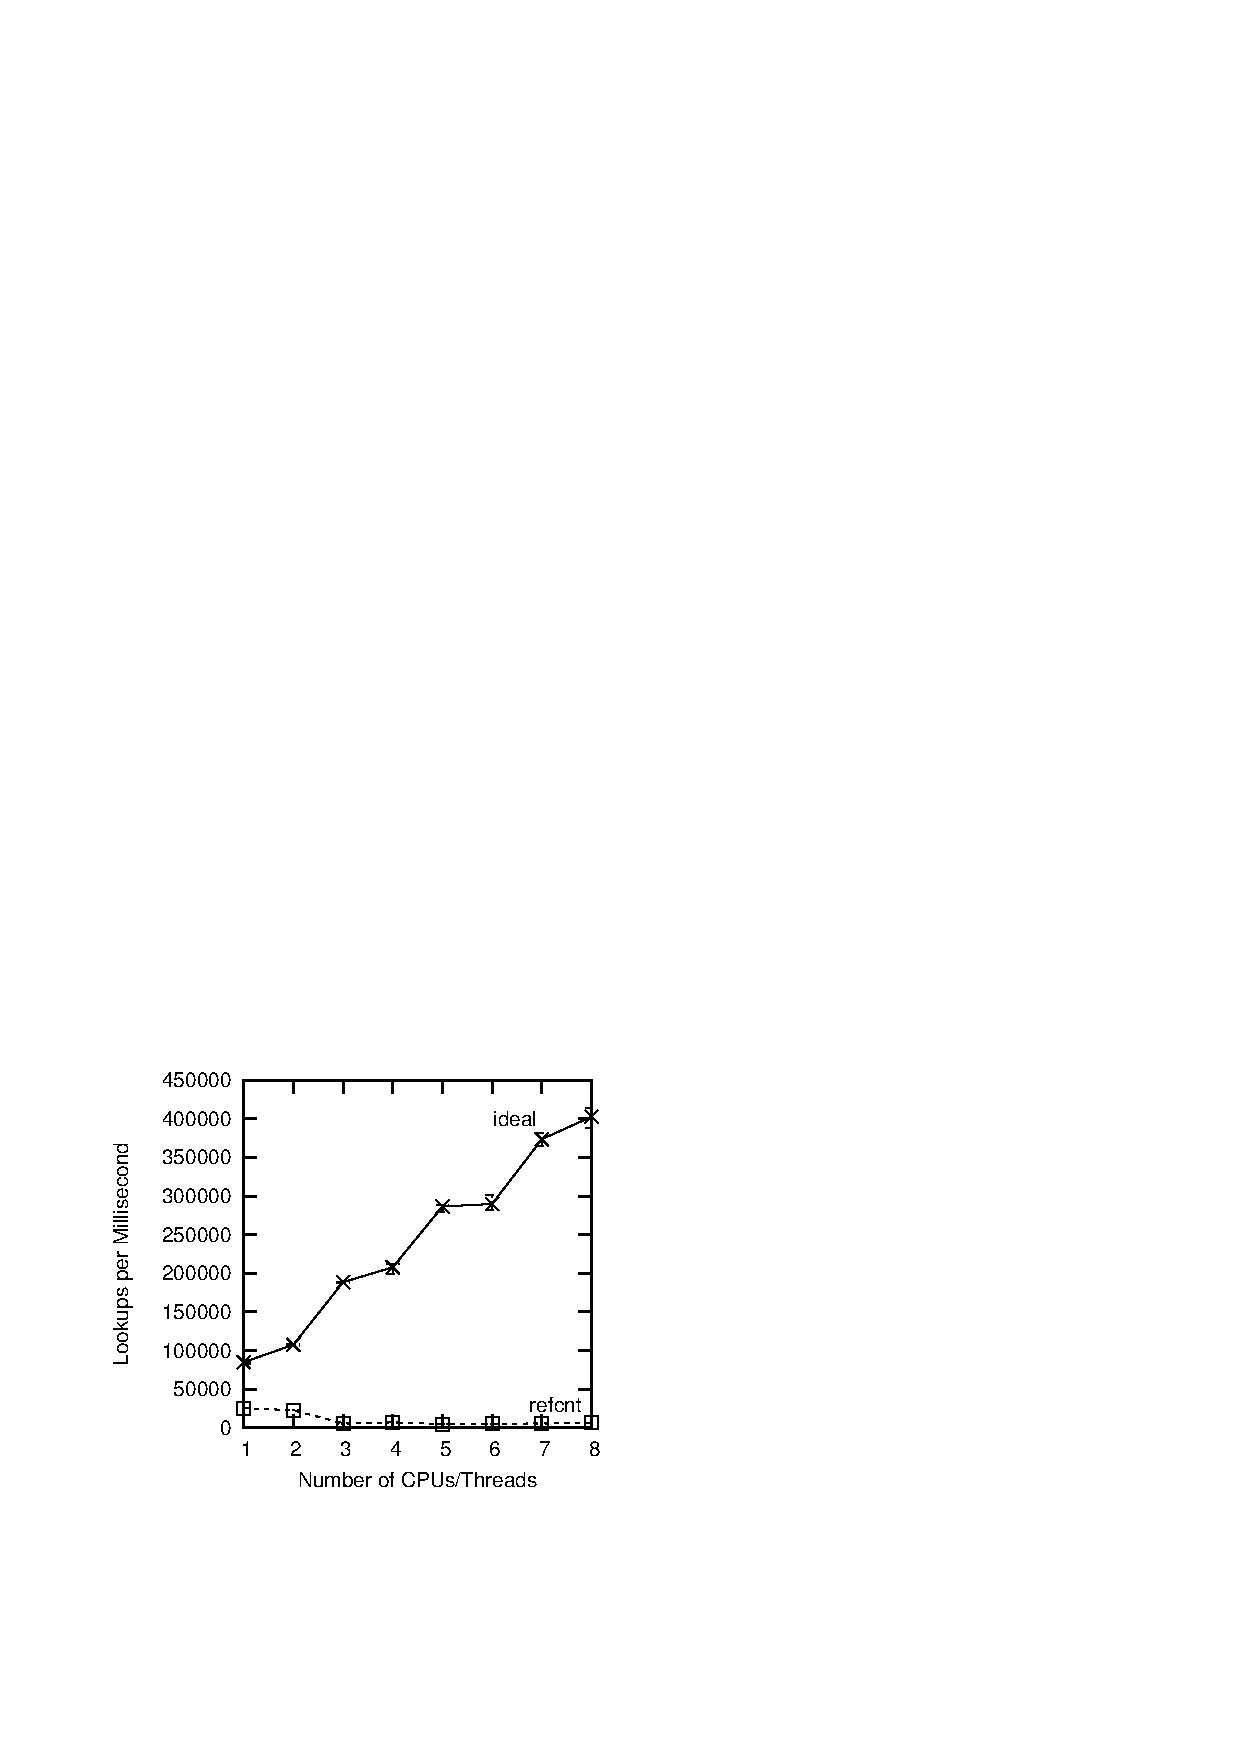
\includegraphics{CodeSamples/defer/data/paulmck.2016/perf-refcnt}}
\caption{Pre-BSD Routing Table Protected by Reference Counting}
\label{fig:defer:Pre-BSD Routing Table Protected by Reference Counting}
\end{figure}

Reference counting tracks the number of references
to a given object in order to prevent that object from being prematurely
freed.

\path{route_refcnt.c}

Although this is a conceptually simple technique, many devils hide in
the details.
After all, if the object was not subject to premature disposal,
there would be no need for the reference counter in the first place.
But if the object can be disposed of, what prevents disposal during
the reference-acquisition process itself?

There are a number of possible answers to this question, including:

\begin{enumerate}
\item	A lock residing outside of the object must be held while
	manipulating the reference count.
\item	The object is created with a non-zero reference count, and new
	references may be acquired only when the current value of
	the reference counter is non-zero.
	If a thread does not have a reference to a given object,
	it may obtain one with the help of another thread that
	already has a reference.
\item	An existence guarantee is provided for the object, preventing
	it from being freed while some other
	entity might be attempting to acquire a reference.
	Existence guarantees are often provided by automatic
	garbage collectors, and, as will be seen in
	Section~\ref{sec:defer:Read-Copy Update (RCU)}, by RCU.
\item	A type-safety guarantee is provided for the object.
	An additional identity check must be performed once
	the reference is acquired.
	Type-safety guarantees can be provided by special-purpose
	memory allocators, for example, by the
	\co{SLAB_DESTROY_BY_RCU} feature within the Linux kernel,
	as will be seen in Section~\ref{sec:defer:Read-Copy Update (RCU)}.
\end{enumerate}

Of course, any mechanism that provides existence guarantees
by definition also provides type-safety guarantees.
This section will therefore group the last two answers together under the
rubric of RCU, leaving us with three general categories of
reference-acquisition protection: Reference counting, sequence
locking, and RCU.

\QuickQuiz{}
	Why not implement reference-acquisition using
	a simple compare-and-swap operation that only
	acquires a reference if the reference counter is
	non-zero?
\QuickQuizAnswer{
	Although this can resolve the race between the release of
	the last reference and acquisition of a new reference,
	it does absolutely nothing to prevent the data structure
	from being freed and reallocated, possibly as some completely
	different type of structure.
	It is quite likely that the ``simple compare-and-swap
	operation'' would give undefined results if applied to the
	differently typed structure.

	In short, use of atomic operations such as compare-and-swap
	absolutely requires either type-safety or existence guarantees.
} \QuickQuizEnd

\begin{table}[tb]
\footnotesize
\centering
\begin{tabular}{l||c|c|c}
	& \multicolumn{3}{c}{Release Synchronization} \\
	\cline{2-4}
	Acquisition     &         & Reference &     \\
	Synchronization & Locking & Counting  & RCU \\
	\hline
	\hline
	Locking		& -	  & CAM	      & CA  \\
	\hline
	Reference	& A	  & AM	      & A   \\
	Counting	&  	  &   	      &     \\
	\hline
	RCU		& CA	  & MCA	      & CA  \\
\end{tabular}
\caption{Reference Counting and Synchronization Mechanisms}
\label{tab:defer:Reference Counting and Synchronization Mechanisms}
\end{table}

Given that the key reference-counting issue
is synchronization between acquisition
of a reference and freeing of the object, we have nine possible
combinations of mechanisms, as shown in
Table~\ref{tab:defer:Reference Counting and Synchronization Mechanisms}.
This table
divides reference-counting mechanisms into the following broad categories:
\begin{enumerate}
\item	Simple counting with neither atomic operations, memory
	barriers, nor alignment constraints \makebox{(``-'')}.
\item	Atomic counting without memory barriers (``A'').
\item	Atomic counting, with memory barriers required only on release
	(``AM'').
\item	Atomic counting with a check combined with the atomic acquisition
	operation, and with memory barriers required only on release
	(``CAM'').
\item	Atomic counting with a check combined with the atomic acquisition
	operation (``CA'').
\item	Atomic counting with a check combined with the atomic acquisition
	operation, and with memory barriers also required on acquisition
	(``MCA'').
\end{enumerate}
However, because all Linux-kernel atomic operations that return a
value are defined to contain memory barriers,\footnote{
	With \co{atomic_read()} and \co{ATOMIC_INIT()} being the
	exceptions that prove the rule.}
all release operations
contain memory barriers, and all checked acquisition operations also
contain memory barriers.
Therefore, cases ``CA'' and ``MCA'' are equivalent to ``CAM'', so that
there are sections below for only the first four cases:
\makebox{``-''}, ``A'', ``AM'', and ``CAM''.
The Linux primitives that support reference counting are presented in
Section~\ref{sec:defer:Linux Primitives Supporting Reference Counting}.
Later sections cite optimizations that can improve performance
if reference acquisition and release is very frequent, and the
reference count need be checked for zero only very rarely.

\subsection{Implementation of Reference-Counting Categories}
\label{sec:defer:Implementation of Reference-Counting Categories}

Simple counting protected by locking (\makebox{``-''}) is described in
Section~\ref{sec:defer:Simple Counting},
atomic counting with no memory barriers (``A'') is described in
Section~\ref{sec:defer:Atomic Counting}
atomic counting with acquisition memory barrier (``AM'') is described in
Section~\ref{sec:defer:Atomic Counting With Release Memory Barrier},
and
atomic counting with check and release memory barrier (``CAM'') is described in
Section~\ref{sec:defer:Atomic Counting With Check and Release Memory Barrier}.

\subsubsection{Simple Counting}
\label{sec:defer:Simple Counting}

Simple counting, with neither atomic operations nor memory barriers,
can be used when the reference-counter acquisition and release are
both protected by the same lock.
In this case, it should be clear that the reference count itself
may be manipulated non-atomically, because the lock provides any
necessary exclusion, memory barriers, atomic instructions, and disabling
of compiler optimizations.
This is the method of choice when the lock is required to protect
other operations in addition to the reference count, but where
a reference to the object must be held after the lock is released.
Figure~\ref{fig:defer:Simple Reference-Count API} shows a simple
API that might be used to implement simple non-atomic reference
counting -- although simple reference counting is almost always
open-coded instead.

{ \scriptsize
\begin{verbbox}
  1 struct sref {
  2   int refcount;
  3 };
  4
  5 void sref_init(struct sref *sref)
  6 {
  7   sref->refcount = 1;
  8 }
  9
 10 void sref_get(struct sref *sref)
 11 {
 12   sref->refcount++;
 13 }
 14
 15 int sref_put(struct sref *sref,
 16              void (*release)(struct sref *sref))
 17 {
 18   WARN_ON(release == NULL);
 19   WARN_ON(release == (void (*)(struct sref *))kfree);
 20
 21   if (--sref->refcount == 0) {
 22     release(sref);
 23     return 1;
 24   }
 25   return 0;
 26 }
\end{verbbox}
}
\begin{figure}[tbp]
\centering
\theverbbox
\caption{Simple Reference-Count API}
\label{fig:defer:Simple Reference-Count API}
\end{figure}

\subsubsection{Atomic Counting}
\label{sec:defer:Atomic Counting}

Simple atomic counting may be used in cases where any CPU acquiring
a reference must already hold a reference.
This style is used when a single CPU creates an object for its
own private use, but must allow other CPU, tasks, timer handlers,
or I/O completion handlers that it later spawns to also access this object.
Any CPU that hands the object off must first acquire a new reference
on behalf of the recipient object.
In the Linux kernel, the \co{kref} primitives are used to implement
this style of reference counting, as shown in
Figure~\ref{fig:defer:Linux Kernel kref API}.

Atomic counting is required
because locking is not used to protect all reference-count operations,
which means that it is possible for two different CPUs to concurrently
manipulate the reference count.
If normal increment and decrement were used, a pair of CPUs might both
fetch the reference count concurrently, perhaps both obtaining
the value ``3''.
If both of them increment their value, they will both obtain ``4'',
and both will store this value back into the counter.
Since the new value of the counter should instead be ``5'', one
of the two increments has been lost.
Therefore, atomic operations must be used both for counter increments
and for counter decrements.

If releases are guarded by locking or RCU,
memory barriers are \emph{not} required, but for different reasons.
In the case of locking, the locks provide any needed memory barriers
(and disabling of compiler optimizations), and the locks also
prevent a pair of releases from running concurrently.
In the case of RCU, cleanup must be deferred until all currently
executing RCU read-side critical sections have completed, and
any needed memory barriers or disabling of compiler optimizations
will be provided by the RCU infrastructure.
Therefore, if two CPUs release the final two references concurrently,
the actual cleanup will be deferred until both CPUs exit their
RCU read-side critical sections.

\QuickQuiz{}
	Why isn't it necessary to guard against cases where one CPU
	acquires a reference just after another CPU releases the last
	reference?
\QuickQuizAnswer{
	Because a CPU must already hold a reference in order
	to legally acquire another reference.
	Therefore, if one CPU releases the last reference,
	there cannot possibly be any CPU that is permitted
	to acquire a new reference.
	This same fact allows the non-atomic check in line~22
	of Figure~\ref{fig:defer:Linux Kernel kref API}.
} \QuickQuizEnd

{ \scriptsize
\begin{verbbox}
  1 struct kref {
  2   atomic_t refcount;
  3 };
  4 
  5 void kref_init(struct kref *kref)
  6 {
  7   atomic_set(&kref->refcount, 1);
  8 }
  9 
 10 void kref_get(struct kref *kref)
 11 {
 12   WARN_ON(!atomic_read(&kref->refcount));
 13   atomic_inc(&kref->refcount);
 14 }
 15 
 16 static inline int
 17 kref_sub(struct kref *kref, unsigned int count,
 18          void (*release)(struct kref *kref))
 19 {
 20   WARN_ON(release == NULL);
 21 
 22   if (atomic_sub_and_test((int) count,
 23                           &kref->refcount)) {
 24     release(kref);
 25     return 1;
 26   }
 27   return 0;
 28 }
\end{verbbox}
}
\begin{figure}[tbp]
\centering
\theverbbox
\caption{Linux Kernel kref API}
\label{fig:defer:Linux Kernel kref API}
\end{figure}

The \co{kref} structure itself, consisting of a single atomic
data item, is shown in lines~1-3 of
Figure~\ref{fig:defer:Linux Kernel kref API}.
The \co{kref_init()} function on lines~5-8 initializes the counter
to the value ``1''.
Note that the \co{atomic_set()} primitive is a simple
assignment, the name stems from the data type of \co{atomic_t}
rather than from the operation.
The \co{kref_init()} function must be invoked during object creation,
before the object has been made available to any other CPU.

The \co{kref_get()} function on lines~10-14 unconditionally atomically
increments the counter.
The \co{atomic_inc()} primitive does not necessarily explicitly
disable compiler
optimizations on all platforms, but the fact that the \co{kref}
primitives are in a separate module and that the Linux kernel build
process does no cross-module optimizations has the same effect.

The \co{kref_put()} function on lines~16-28 atomically decrements the
counter, and if the result is zero, line~24 invokes the specified
\co{release()} function and line~24 returns, informing the caller
that \co{release()} was invoked.
Otherwise, \co{kref_put()} returns zero, informing the caller that
\co{release()} was not called.

\QuickQuiz{}
	Suppose that just after the \co{atomic_sub_and_test()}
	on line~22 of
	Figure~\ref{fig:defer:Linux Kernel kref API} is invoked,
	that some other CPU invokes \co{kref_get()}.
	Doesn't this result in that other CPU now having an illegal
	reference to a released object?
\QuickQuizAnswer{
	This cannot happen if these functions are used correctly.
	It is illegal to invoke \co{kref_get()} unless you already
	hold a reference, in which case the \co{kref_sub()} could
	not possibly have decremented the counter to zero.
} \QuickQuizEnd

\QuickQuiz{}
	Suppose that \co{kref_sub()} returns zero, indicating that
	the \co{release()} function was not invoked.
	Under what conditions can the caller rely on the continued
	existence of the enclosing object?
\QuickQuizAnswer{
	The caller cannot rely on the continued existence of the
	object unless it knows that at least one reference will
	continue to exist.
	Normally, the caller will have no way of knowing this, and
	must therefore carefullly avoid referencing the object after
	the call to \co{kref_sub()}.
} \QuickQuizEnd

\QuickQuiz{}
	Why not just pass \co{kfree()} as the release function?
\QuickQuizAnswer{
	Because the \co{kref} structure normally is embedded in
	a larger structure, and it is necessary to free the entire
	structure, not just the \co{kref} field.
	This is normally accomplished by defining a wrapper function
	that does a \co{container_of()} and then a \co{kfree()}.
} \QuickQuizEnd

\subsubsection{Atomic Counting With Release Memory Barrier}
\label{sec:defer:Atomic Counting With Release Memory Barrier}

This style of reference is used in the Linux kernel's networking
layer to track the destination caches that are used in packet routing.
The actual implementation is quite a bit more involved; this section
focuses on the aspects of \co{struct dst_entry} reference-count
handling that matches this use case,
shown in Figure~\ref{fig:defer:Linux Kernel dst-clone API}.

{ \scriptsize
\begin{verbbox}
  1 static inline
  2 struct dst_entry * dst_clone(struct dst_entry * dst)
  3 {
  4   if (dst)
  5     atomic_inc(&dst->__refcnt);
  6   return dst;
  7 }
  8
  9 static inline
 10 void dst_release(struct dst_entry * dst)
 11 {
 12   if (dst) {
 13     WARN_ON(atomic_read(&dst->__refcnt) < 1);
 14     smp_mb__before_atomic_dec();
 15     atomic_dec(&dst->__refcnt);
 16   }
 17 }
\end{verbbox}
}
\begin{figure}[tbp]
\centering
\theverbbox
\caption{Linux Kernel dst\_clone API}
\label{fig:defer:Linux Kernel dst-clone API}
\end{figure}

The \co{dst_clone()} primitive may be used if the caller
already has a reference to the specified \co{dst_entry},
in which case it obtains another reference that may be handed off
to some other entity within the kernel.
Because a reference is already held by the caller, \co{dst_clone()}
need not execute any memory barriers.
The act of handing the \co{dst_entry} to some other entity might
or might not require a memory barrier, but if such a memory barrier
is required, it will be embedded in the mechanism used to hand the
\co{dst_entry} off.

The \co{dst_release()} primitive may be invoked from any environment,
and the caller might well reference elements of the \co{dst_entry}
structure immediately prior to the call to \co{dst_release()}.
The \co{dst_release()} primitive therefore contains a memory
barrier on line~14 preventing both the compiler and the CPU
from misordering accesses.

Please note that the programmer making use of \co{dst_clone()} and
\co{dst_release()} need not be aware of the memory barriers, only
of the rules for using these two primitives.

\subsubsection{Atomic Counting With Check and Release Memory Barrier}
\label{sec:defer:Atomic Counting With Check and Release Memory Barrier}

Consider a situation where the caller must be able to acquire a new
reference to an object to which it does not already hold a reference.
The fact that initial reference-count acquisition can now run concurrently
with reference-count release adds further complications.
Suppose that a reference-count release finds that the new
value of the reference count is zero, signalling that it is
now safe to clean up the reference-counted object.
We clearly cannot allow a reference-count acquisition to
start after such clean-up has commenced, so the acquisition
must include a check for a zero reference count.
This check must be part of the atomic increment operation,
as shown below.

\QuickQuiz{}
	Why can't the check for a zero reference count be
	made in a simple ``if'' statement with an atomic
	increment in its ``then'' clause?
\QuickQuizAnswer{
	Suppose that the ``if'' condition completed, finding
	the reference counter value equal to one.
	Suppose that a release operation executes, decrementing
	the reference counter to zero and therefore starting
	cleanup operations.
	But now the ``then'' clause can increment the counter
	back to a value of one, allowing the object to be
	used after it has been cleaned up.
} \QuickQuizEnd

The Linux kernel's \co{fget()} and \co{fput()} primitives
use this style of reference counting.
Simplified versions of these functions are shown in
Figure~\ref{fig:defer:Linux Kernel fget/fput API}.

{ \fontsize{6.5pt}{7.5pt}\selectfont
\begin{verbbox}
  1 struct file *fget(unsigned int fd)
  2 {
  3   struct file *file;
  4   struct files_struct *files = current->files;
  5
  6   rcu_read_lock();
  7   file = fcheck_files(files, fd);
  8   if (file) {
  9     if (!atomic_inc_not_zero(&file->f_count)) {
 10       rcu_read_unlock();
 11       return NULL;
 12     }
 13   }
 14   rcu_read_unlock();
 15   return file;
 16 }
 17
 18 struct file *
 19 fcheck_files(struct files_struct *files, unsigned int fd)
 20 {
 21   struct file * file = NULL;
 22   struct fdtable *fdt = rcu_dereference((files)->fdt);
 23
 24   if (fd < fdt->max_fds)
 25     file = rcu_dereference(fdt->fd[fd]);
 26   return file;
 27 }
 28
 29 void fput(struct file *file)
 30 {
 31   if (atomic_dec_and_test(&file->f_count))
 32     call_rcu(&file->f_u.fu_rcuhead, file_free_rcu);
 33 }
 34
 35 static void file_free_rcu(struct rcu_head *head)
 36 {
 37   struct file *f;
 38
 39   f = container_of(head, struct file, f_u.fu_rcuhead);
 40   kmem_cache_free(filp_cachep, f);
 41 }
\end{verbbox}
}
\begin{figure}[tbp]
\centering
\theverbbox
\caption{Linux Kernel fget/fput API}
\label{fig:defer:Linux Kernel fget/fput API}
\end{figure}

Line~4 of \co{fget()} fetches the pointer to the current
process's file-descriptor table, which might well be shared
with other processes.
Line~6 invokes \co{rcu_read_lock()}, which
enters an RCU read-side critical section.
The callback function from any subsequent \co{call_rcu()} primitive
will be deferred until a matching \co{rcu_read_unlock()} is reached
(line~10 or 14 in this example).
Line~7 looks up the file structure corresponding to the file
descriptor specified by the \co{fd} argument, as will be
described later.
If there is an open file corresponding to the specified file descriptor,
then line~9 attempts to atomically acquire a reference count.
If it fails to do so, lines~10-11 exit the RCU read-side critical
section and report failure.
Otherwise, if the attempt is successful, lines~14-15 exit the read-side
critical section and return a pointer to the file structure.

The \co{fcheck_files()} primitive is a helper function for
\co{fget()}.
It uses the \co{rcu_dereference()} primitive to safely fetch an
RCU-protected pointer for later dereferencing (this emits a
memory barrier on CPUs such as DEC Alpha in which data dependencies
do not enforce memory ordering).
Line~22 uses \co{rcu_dereference()} to fetch a pointer to this
task's current file-descriptor table,
and line~24 checks to see if the specified file descriptor is in range.
If so, line~25 fetches the pointer to the file structure, again using
the \co{rcu_dereference()} primitive.
Line~26 then returns a pointer to the file structure or \co{NULL}
in case of failure.

The \co{fput()} primitive releases a reference to a file structure.
Line~31 atomically decrements the reference count, and, if the result
was zero, line~32 invokes the \co{call_rcu()} primitives in order to
free up the file structure (via the \co{file_free_rcu()} function
specified in \co{call_rcu()}'s second argument),
but only after all currently-executing
RCU read-side critical sections complete.
The time period required for all currently-executing RCU read-side
critical sections to complete is termed a ``grace period''.
Note that the \co{atomic_dec_and_test()} primitive contains
a memory barrier.
This memory barrier is not necessary in this example, since the structure
cannot be destroyed until the RCU read-side critical section completes,
but in Linux, all atomic operations that return a result must
by definition contain memory barriers.

Once the grace period completes, the \co{file_free_rcu()} function
obtains a pointer to the file structure on line~39, and frees it
on line~40.

This approach is also used by Linux's virtual-memory system,
see \co{get_page_unless_zero()} and \co{put_page_testzero()} for
page structures as well as \co{try_to_unuse()} and \co{mmput()}
for memory-map structures.

\subsection{Linux Primitives Supporting Reference Counting}
\label{sec:defer:Linux Primitives Supporting Reference Counting}

The Linux-kernel primitives used in the above examples are
summarized in the following list.
\IfInBook{}{The RCU primitives may be unfamiliar to some readers,
	    so a brief overview with citations is included in
	    Section~\ref{sec:defer:Background on RCU}.}

\begin{itemize}
\item	\co{atomic_t}
	Type definition for 32-bit quantity to be manipulated atomically.
\item	\co{void atomic_dec(atomic_t *var);}
	Atomically decrements the referenced variable without necessarily
	issuing a memory barrier or disabling compiler optimizations.
\item	\co{int atomic_dec_and_test(atomic_t *var);}
	Atomically decrements the referenced variable, returning
	\co{true} (non-zero) if the result is zero.
	Issues a memory barrier and disables compiler optimizations that
	might otherwise move memory references across this primitive.
\item	\co{void atomic_inc(atomic_t *var);}
	Atomically increments the referenced variable without necessarily
	issuing a memory barrier or disabling compiler optimizations.
\item	\co{int atomic_inc_not_zero(atomic_t *var);}
	Atomically increments the referenced variable, but only if the
	value is non-zero, and returning \co{true} (non-zero) if the
	increment occurred.
	Issues a memory barrier and disables compiler optimizations that
	might otherwise move memory references across this primitive.
\item	\co{int atomic_read(atomic_t *var);}
	Returns the integer value of the referenced variable.
	This need not be an atomic operation, and it need not issue any
	memory-barrier instructions.
	Instead of thinking of as ``an atomic read,'' think of it as
	``a normal read from an atomic variable.''
\item	\co{void atomic_set(atomic_t *var, int val);}
	Sets the value of the referenced atomic variable to ``val''.
	This need not be an atomic operation, and it is not required
	to either issue memory
	barriers or disable compiler optimizations.
	Instead of thinking of as ``an atomic set,'' think of it as
	``a normal set of an atomic variable.''
\item	\co{void call_rcu(struct rcu_head *head, void (*func)(struct rcu_head *head));}
	Invokes \co{func(head)} some time after all currently executing RCU
	read-side critical sections complete, however, the \co{call_rcu()}
	primitive returns immediately.
	Note that \co{head} is normally a field within an RCU-protected
	data structure, and that \co{func} is normally a function that
	frees up this data structure.
	The time interval between the invocation of \co{call_rcu()} and
	the invocation of \co{func} is termed a ``grace period''.
	Any interval of time containing a grace period is itself a
	grace period.
\item	\co{type *container_of(p, type, f);}
	Given a pointer \co{p} to a field \co{f} within a structure
	of the specified type, return a pointer to the structure.
\item	\co{void rcu_read_lock(void);}
	Marks the beginning of an RCU read-side critical section.
\item	\co{void rcu_read_unlock(void);}
	Marks the end of an RCU read-side critical section.
	RCU read-side critical sections may be nested.
\item	\co{void smp_mb__before_atomic_dec(void);}
	Issues a memory barrier and disables code-motion compiler
	optimizations only if the platform's \co{atomic_dec()}
	primitive does not already do so.
\item	\co{struct rcu_head}
	A data structure used by the RCU infrastructure to track
	objects awaiting a grace period.
	This is normally included as a field within an RCU-protected
	data structure.
\end{itemize}

\QuickQuiz{}
	An \co{atomic_read()} and an \co{atomic_set()} that are
	non-atomic?
	Is this some kind of bad joke???
\QuickQuizAnswer{
	It might well seem that way, but in situations where no other
	CPU has access to the atomic variable in question, the overhead
	of an actual atomic instruction would be wasteful.
	Two examples where no other CPU has access are
	during initialization and cleanup.
} \QuickQuizEnd

\subsection{Counter Optimizations}
\label{sec:defer:Counter Optimizations}

In some cases where increments and decrements are common, but checks
for zero are rare, it makes sense to maintain per-CPU or per-task
counters, as was discussed in Chapter~\ref{chp:Counting}.
See the paper on sleepable read-copy update
(SRCU) for an example of this technique applied to
RCU~\cite{PaulEMcKenney2006c}.
This approach eliminates the need for atomic instructions or memory
barriers on the increment and decrement primitives, but still requires
that code-motion compiler optimizations be disabled.
In addition, the primitives such as \co{synchronize_srcu()}
that check for the aggregate reference
count reaching zero can be quite slow.
This underscores the fact that these techniques are designed
for situations where the references are frequently acquired and
released, but where it is rarely necessary to check for a zero
reference count.

% @@@ Difficulty of managing reference counts: leaks, premature freeing.

However, it is usually the case that use of reference counts requires
writing (often atomically) to a data structure that is otherwise
read only.
In this case, reference counts are imposing expensive cache misses
on readers.

It is therefore worthwhile to look into synchronization mechanisms
that do not require readers to write to the data structure being
traversed.
One such synchronization mechanism, hazard pointers, is covered in
the next section.
